\documentclass[10pt,fleqn]{article}

\usepackage{graphicx}
\usepackage{graphics}
\usepackage{multicol}
\usepackage{epsfig,amsmath,amsfonts}
\usepackage{xspace}
\usepackage{url}
\usepackage{subfigure}

\makeatletter                                   % Make '@' accessible. 
\oddsidemargin=0in                              % Left margin minus 1 inch.
\evensidemargin=0in                             % Same for even-numbered pages.
\marginparsep=0pt                               % Space between margin & text

\renewcommand{\baselinestretch}{1.2}              % Double spacing

\textwidth=6.5in                                % Text width (8.5in - margins).
\textheight=9in                                 % Body height (incl. footnotes)

\topmargin=0in                                  % Top margin minus 1 inch.
\headsep=0.0in                                  % Distance from header to body.
\skip\footins=4ex                               % Space above first footnote.
\hbadness=10000                                 % No "underfull hbox" messages.
\makeatother                                    % Make '@' special again.

\def\sim{TOSSIM\xspace}
\def\tinyviz{TinyViz\xspace}
\def\mote{mote\xspace}
\def\motes{motes\xspace}
\def\Mote{Mote\xspace}
\def\Motes{Motes\xspace}

\begin{document}

\fontfamily{cmss}                               % Make text sans serif.
\fontseries{m}                                  % Medium spacing.
\fontshape{n}                                   % Normal: not bold, etc.
\fontsize{10}{10}                               % 10pt font, 10pt line spacing 

\title{\vspace{2.5in}\sim: A Simulator for TinyOS Networks}
\author{Philip Levis and Nelson Lee\\ pal@cs.berkeley.edu}

\maketitle
\vspace{2in}
\begin{center}
Version 1.0\\
June 26, 2003
\end{center}
\newpage

\fontfamily{cmr}                                % Make text Roman (serif).
\fontseries{m}                                  % Medium spacing.
\fontshape{n}                                   % Normal: not bold, etc.
\fontsize{10}{10}                               % 10pt font, 10pt line spacing

\tableofcontents

\section{Introduction}

\sim is a discrete event simulator for TinyOS sensor
networks. Instead of compiling a TinyOS application for a mote, users
can compile it into the \sim framework, which runs on a PC. This
allows users to debug, test, and analyze algorithms in a controlled
and repeatable environment. As \sim runs on a PC, users can examine
their TinyOS code using debuggers and other development tools. This
document briefly describes the design philosophy of
\sim, its capabilities, its structure. It also provides a brief
tutorial on how to use \sim for testing or analysis.

\sim's primary goal is to provide a high fidelity simulation of TinyOS
applications. For this reason, it focuses on simulating TinyOS and its
execution, rather than simulating the real world. While \sim can be
used to understand the causes of behavior observed in the real world,
it does not capture all of them, and should not be used for absolute
evaluations.

\sim is not always the right simulation solution; like any
simulation, it makes several assumptions, focusing on making some
behaviors accurate while simplying others. One of the most common
questions about \sim is whether it can ``simulate X'' or whether it
``has an accurate X model.'' In hope of answering most of such
questions, here is a brief summmary of its characteristics:

\begin{itemize}

\item{\bf Fidelity:} By default, \sim captures TinyOS' behavior at a
very low level. It simulates the network at the bit level, simulates
each individual ADC capture, and every interrupt in the system.

\item{\bf Time:} While \sim precisely times interrupts (allowing
things like bit-level radio simulation), it does not model execution
time. From \sim's perspective, a piece of code runs
instantaneously. Time is kept at a 4MHz granularity (the CPU clock
rate of the rene and mica platforms). This also means that spin locks
or task spin locks will never exit: as the code runs instantaneously,
the event that would allow the spin to stop will not occur until the
code completes (never).

\item{\bf Models:} \sim itself does not model the real world. Instead,
it provides abstractions of certain real-world phenomena (such as bit
error). With tools outside the simulation itself, users can then
manipulate these abstractions to implement whatever models they want
to use. By making complex models exterior to the simulation, \sim
remains flexible to the needs of many users without trying to
establish what is ``correct.'' Additionally, it keeps the simulation
simple and efficient.

\begin{itemize}
\item{\bf Radio:} \sim does not model radio propagation;
instead, it provides a radio abstraction of directed independent bit
errors between two nodes. An external program can provide a desired
radio model and map it to these bit errors. Having directed bit error
rates means that asymmetric links can be easily modeled. Independent
bit errors mean longer packets have a higher probability of
corruption, and each packet's loss probability is independent.

\item{\bf Power/Energy:} \sim does not model power draw or energy
consumption. However, it is very simple to add annotations to
components that consume power to provide information on when their
power states change (e.g., turned on or off). After a simulation is
run, a user can apply a energy or power model to these transitions,
calculating overall energy consumption. Because \sim does not model
CPU execution time, it cannot easily provide accurate information for
calculating CPU energy consumption.
\end{itemize}

\item{\bf Building:} \sim builds directly from TinyOS code. To simulate
a protocol or system, you must write a TinyOS implementation of it. On
one hand, this is often more difficult than an abstract simulation; on
the other, it means you can then take your implementation and run it
on actual motes.

\item{\bf Imperfections:} Although \sim captures TinyOS
behavior at a very low level, it makes several simplifying
assumptions. This means that it is very possible that code which runs
in a simulation might not run on a real mote. For example, in \sim
interrupts are non-preemptive (a result of being a discrete event
simulator). On a real mote, an interrupt can fire while other code is
running. If pre-emption can put a mote in an unrecoverable state, then
simulated motes will run without mishap while real-world motes may
fail. Also, if interrupt handlers run too long, a real-world mote may
crash; as code in \sim runs instantaneously, no problems will appear
in simulation. 

\item{\bf Networking:} Currently, \sim simulates the 40Kbit RFM mica
networking stack, including the MAC, encoding, timing, and synchronous
acknowledgements. It does not simulate the mica2 ChipCon CC1000 stack.
We are waiting to have a better understanding of the behavior of
CC1000 before writing a simulation implementation.

\item{\bf Authority:} Initial experience from real-world deployments has shown
that TinyOS networks have very complex and highly variable behavior.
While \sim is useful to get a sense of how algorithms perform in
comparison to one another, \sim results shouldn't be considered
authoritative. For example, \sim can tell you that one algorithm
behaves better than another under high loss, but the question remains
as to whether the specified loss scenario has any basis in the real
world. \sim should not be considered an end-point of evaluation;
instead, it is a system that allows the user to separate out
environmental noise to better understand algortithms.

\end{itemize}

\section{Compiling and Running a Simulation}

\sim is automatically built when you compile an
application. Applications are compiled by entering an application
directory (e.g. {\tt /apps/Blink}) and typing {\tt
make}. Alternatively, when in an application directory, you can type
{\tt make pc}, which will only compile a simulation of the
application.

There are several compilation options to {\tt ncc} when compiling for
TOSSIM, including the maximum number of motes that can be
simulated. The default options in the TinyOS 1.1 makefile should fit
almost any need; refer to the nesC manual for further information on
the options available.

The \sim executable is named {\tt main.exe}, and resides in {\tt
build/pc}. It has the following usage:

\begin{verbatim}
Usage: ./build/pc/main.exe [options] num_nodes
  [options] are:
  -h, --help        Display this message.
  -gui              pauses simulation waiting for GUI to connect
  -a=<model>        specifies ADC model (generic is default)
                    options: generic random
  -b=<sec>          motes boot over first <sec> seconds (default: 10)
  -ef=<file>        use <file> for eeprom; otherwise anonymous file is used
  -l=<scale>        run sim at <scale> times real time (fp constant)
  -r=<model>        specifies a radio model (simple is default)
                    options: simple static lossy
  -rf=<file>        specifies file input for lossy model (lossy.nss is default)
  -s=<num>          only boot <num> of nodes
  -t=<sec>          run simulation for <sec> virtual seconds
  num_nodes         number of nodes to simulate
\end{verbatim}

The {\tt -h} or {\tt --help} options prints out the above usage
message, and some additional information.

The {\tt -a} option specifies the ADC model to use. \sim currently
supports two models: generic and random. Section~\ref{sec:adc}
describes these models.

The {\tt -b} option specifies the interval over which motes
boot. Their boot times are uniformly distributed over this
interval. The default value is ten seconds.

The {\tt -e} option is for named EEPROM files. If {\tt -e} isn't
specified, the logger component stores and reads data, but this data
is not persistent across simulator invocations: it uses an anonymous
file. Section~\ref{sec:eeprom} describes how the EEPROM in \sim works.

The {\tt -l} option is for making \sim run at a rate representative of
real time. The {\tt scale} argument specifies what relative rate
should be used. For example, {\tt -l=2.0} means twice as fast as real
time (two virtual seconds run in one real second), while {\tt -l=0.1}
means one tenth of real time (one virtual seconds runs in ten real
seconds.). \sim can only run so fast; specifying it to run faster than
it can will cause it to run as quickly as possible. Using this option
imposes a significant performance overhead; it shouldn't be used when
trying to run simulations quickly.

The {\tt -r} option specifies the radio model to use. \sim currently
supports two models: simple and lossy. Earlier versions also supported
a ``static'' model, but this has been subsumed by the lossy
model. Section~\ref{sec:radio} describes these models

The {\tt -s} option tells \sim to only boot a subset of the number of
nodes specified. This is useful if you want some to boot later, in
response to user input. If the {\tt -s} option is specified, \sim
boots mote IDs 0-{\tt (num - 1)}.

The {\tt -t} option tells \sim to run for a specified number of
virtual seconds. After {\tt sec} seconds have passed, \sim exits cleanly.

The {\tt num\_nodes} option specifies how many nodes should be
simulated. A compile-time upper bound is specified in {\tt
/apps/Makerules}. The standard TinyOS distribution sets this value to
be 1000. By default, all {\tt num\_nodes} boot in the first ten
seconds of simulation, with bootup times uniformly distributed.

\sim catches SIGINT (control-C) to exit cleanly. This is useful when
profiling code.

\subsection{dbg}

\sim provides configuration of debugging output at run-time. Much of the
TinyOS source contains debugging statements. Each debugging statement
is accompanied by one or more modal flags. When the simulator starts,
it reads in the DBG environment variable to determine which modes
should be enabled. Modes are stored and processed as entries in a
bit-mask, so a single output can be enabled for multiple modes, and a
user can specify multiple modes to be displayed. The set of DBG modes
recognized by \sim can be identified by using the {\tt -h} option; all
available modes are printed. The current modes are:

\scriptsize
\vspace{0.2in}
\begin{tabular}{ll}
all:      & Enable all available messages \\
boot:     & Simulation boot and StdControl\\
clock:    & The hardware clock\\
task:     & Task enqueueing/dequeueing/running\\
sched:    & The TinyOS scheduler\\
sensor:   & Sensor readings \\
led:      & Mote leds\\
crypto:   & Cryptographic operations (e.g., TinySec)\\
route:    & Routing systems\\
am:       & Active messages transmission/reception\\
crc:      & CRC checks on active messages\\
packet:   & Packet-level transmission/reception\\
encode:   & Packet encoding/decoding\\
radio:    & Low-level radio operations: bits and bytes\\
logger:   & Non-volatile storage\\
adc:      & The ADC \\
i2c:      & The I2C bus\\
uart:     & The UART (serial port)\\
prog:     & Network reprogramming\\
sounder:  & The sounder on the mica sensor board\\
time:     & Timers\\
sim:      & \sim internals\\
queue:    & \sim event queue\\
simradio: & \sim radio models\\
hardware: & \sim hardware abstractions\\
simmem:   & \sim memory allocation/deallocation (for finding leaks)\\
usr1:     & User output mode 1\\
usr2:     & User output mode 2\\
usr3:     & User output mode 3\\
temp:     & For temporary use\\
\end{tabular}
\vspace{0.2in}
\normalsize

As an example, the statement

\scriptsize
\begin{verbatim}
        dbg(DBG_CRC, "crc check failed: \%x, \%x\n", crc, mcrc);
\end{verbatim}
\normalsize

\noindent will print out the failed CRC check message if the user has enabled
CRC debug messages, while

\scriptsize
\begin{verbatim}
        dbg(DBG_BOOT, "AM Module initialized\n");
\end{verbatim}
\normalsize

\noindent will be printed to standard out if boot messages are enabled. DBG
flags can also be combined, as in this example:

\scriptsize
\begin{verbatim}
        dbg(DBG_ROUTE|DBG_ERROR, "Received control message: lose our network name!.\n");
\end{verbatim}
\normalsize

\noindent This will print out if either route or error messages are enabled.

There are a set of bindings from ASCII strings to debug modes. For
example, setting DBG to ``{\tt boot}'' will enable boot message (by
setting the appropriate bit in the mask). Setting DBG to ``{\tt
boot,route,am}''\footnote{E.g. ``{\tt export DBG=boot,route,am}'' in bash,
``{\tt setenv DBG boot,route,am}'' in tcsh, etc.} will enable boot,
routing and active message output. Generally, the name of the flag in
TinyOS source is ``{\tt DBG\_}'', followed by the name of the DBG
option in all caps. For example, the environment variable value ``{\tt
am}'' enables {\tt DBG\_AM} messages, and the value ``{\tt usr1}''
enables {\tt DBG\_USR1} messages. Note that if you don't set DBG, then all
debug output is enabled and the simulation will run very slowly.

Four modes are reserved for application components: usr1, usr2, usr3,
and temp. Developers are urged to use these modes in their code. When
TinyOS is compiled for mote hardware, all of debug statements are
removed; we have verified that they add no instructions to the TinyOS
code image.

We have found one of the easiest way to run experiments and gather
data is to use dbg statements and save them to a file. Generally, the
more data printed out, the better (to a point); Perl scripts or other
tools can then read in the log of the run and provide information on
packet loss rates, routing state, etc. A useful function, defined in
{\tt external\_comm.c}, is {\tt printTime(char* buf, int len)}. It
takes the current time in simulation and converts it to the form
HH:MM:SS, putting it in {\tt buf}..

\subsection{Network Monitoring and Packet Injection}

To interact with a simulated network, you must use SerialForwarder,
the standard TinyOS interface tool. To work with \sim,
SerialForwarder's input source must be set appropriately. \sim
provides two modes: communication through a serial port to mote 0
and network snooping.

The serial port mode (``tossim-serial'' in the ``Mote Communications''
field or ``-comm tossim-serial'' at the command line) interacts with mote 0
over its serial port. Programs connecting to SerialForwarder can read
messages mote 0 sends to its serial port, and send messages to mote 0 over
its serial port.

The snooping mode (``tossim-radio'' in the ``Mote Communications'' field
or ``-comm tossim-radio'' at the command line) sits on top of the \sim
network model. Programs connecting to SerialForwarder hear every radio
message sent in the network, and can inject radio messages to arrive
(without error) at any mote. Because this mode outputs every message {\it
sent}, it does not consider loss; programs connecting will hear packets
that might not arrive successfully at any mote.

It's often helpful to use the {\tt -l} flag when using the serial port
mode; external applications can then interact with a network in
something approximating real time. Otherwise, in simulations of small
numbers of motes, things like network timeouts can go off before a PC
application has a chance to respond.

Message Interface Generator (MIG) is a tool that generates Java
classes for TinyOS packets. The MIG tool parses C structures for
TinyOS packets and builds a Java class with accessors for each of the
packet fields. The message classes can also unpack from and pack to
byte arrays.

Using MIG with \sim has one hitch; you must specify the {\tt
-target=pc} flag when compiling your message classes. MIG classes
generated for motes may not work with \sim; the two platforms do not
necessarily pack messages identically. Having different word
boundaries (one byte on motes, four bytes on PCs) means that
structures will have different padding. Problems will definitely
appear if message structures use platform-dependent types such as {\tt
int}. 

\section{Radio Models}
\label{sec:radio}

\sim simulates the TinyOS network at the bit level, using TinyOS
component implementations almost identical to the mica 40Kbit
RFM-based stack. \sim provides two radio models: simple and lossy. The
mica2 CC1000-based stack does not currently have a simulation
implementation.

In \sim, a network signal is either a one or zero. All signals are of
equal strength, and collision is modeled as a logical or; there is no
cancellation. This means that distance does not effect signal
strength; if mote B is very close to mote A, it cannot cut through the
signal from far-away mote C. This makes interference in \sim generally
worse than expected real world behavior.

The ``simple'' radio model places all nodes in a single cell. Every
bit transmitted is received without error. Although no bits are
corrupted due to error, two motes can transmit at the same time; every
mote in the cell will hear the overlap of the signals, which will
almost certainly be a corrupted packet. However, because of perfect
bit transmission in a single cell, the probability of two motes
transmitting at the same time is very, very low, due to the TinyOS
CSMA protocol.

The simple model is useful for testing single-hop algorithms and
TinyOS components for correctness. Deterministic packet reception
allows deterministic results.

\begin{figure}
\centering
\subfigure[Empirical] {\centering
\label{fig:loss_empirical}
          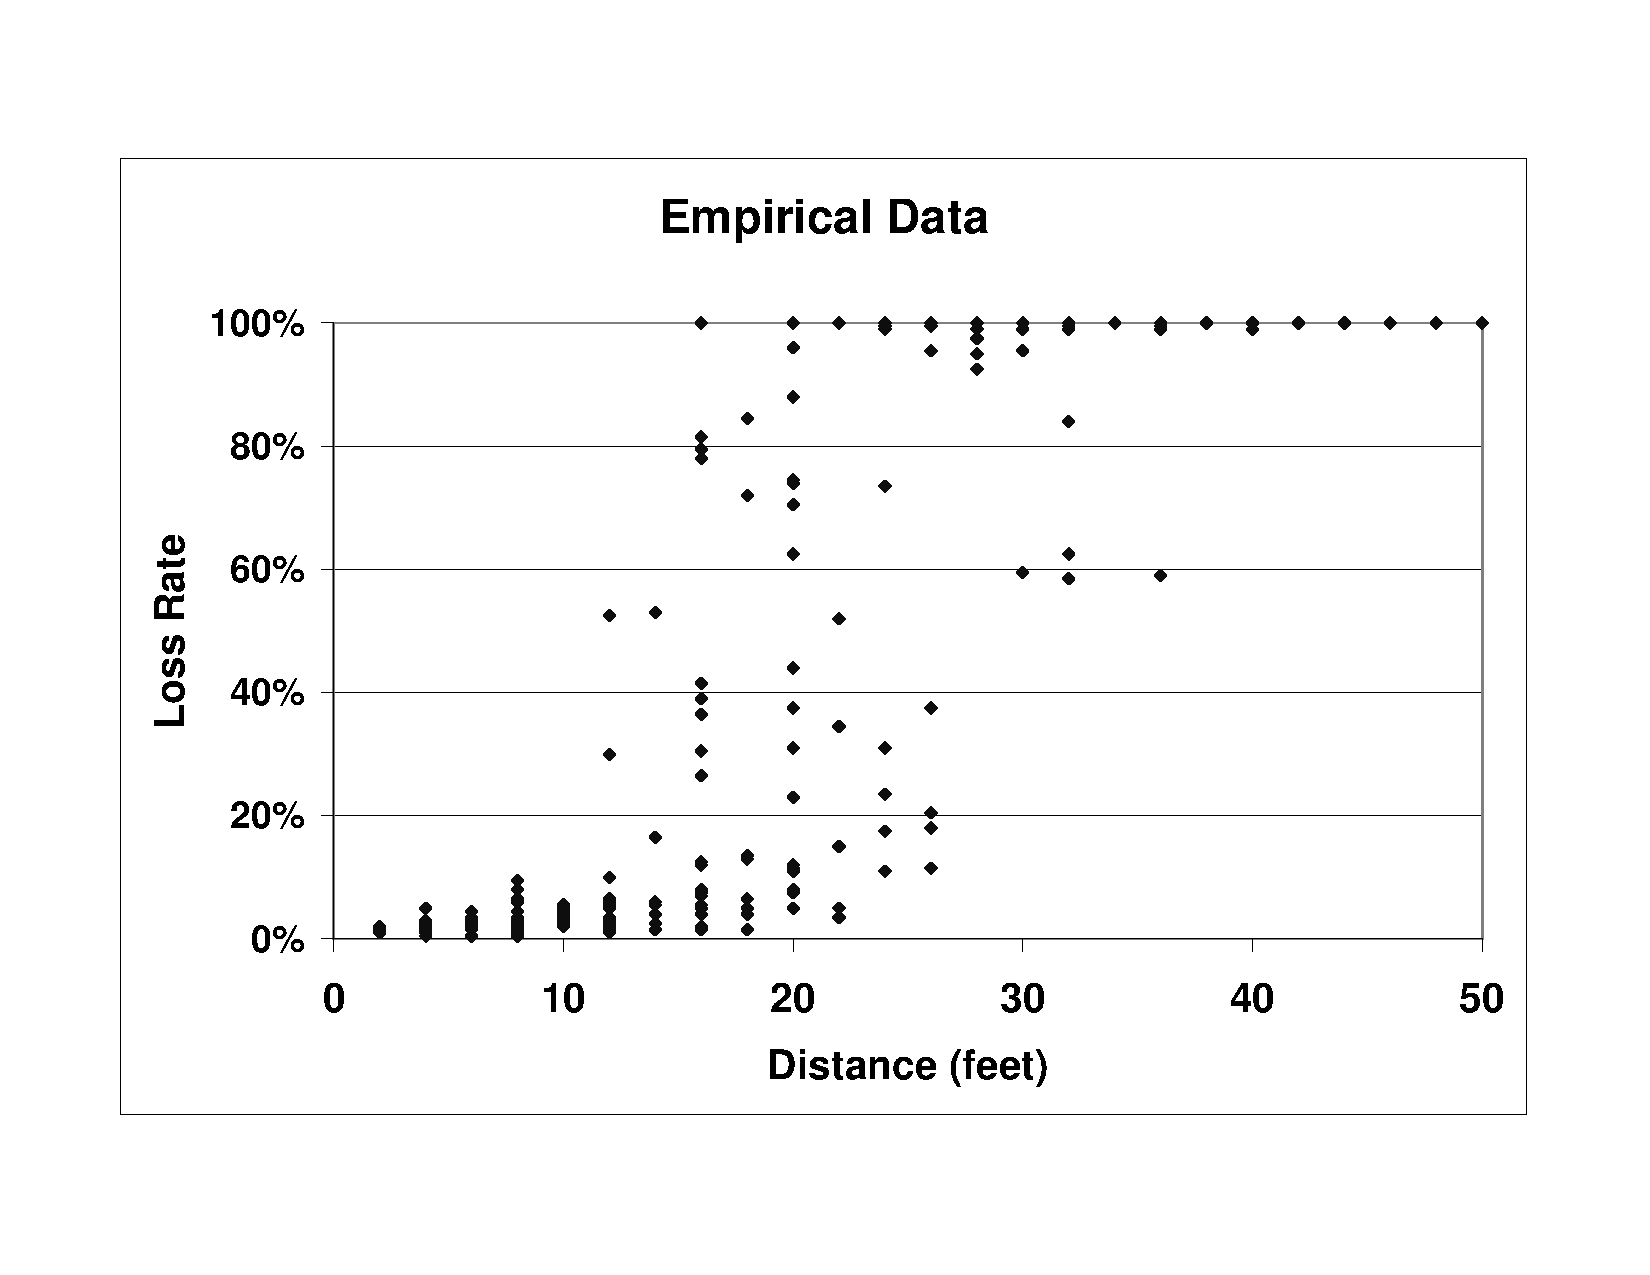
\includegraphics[clip,angle=-90,width=2in]{fig/empirical.pdf}}
\subfigure[Simulated] {\centering
\label{fig:loss_sim}
          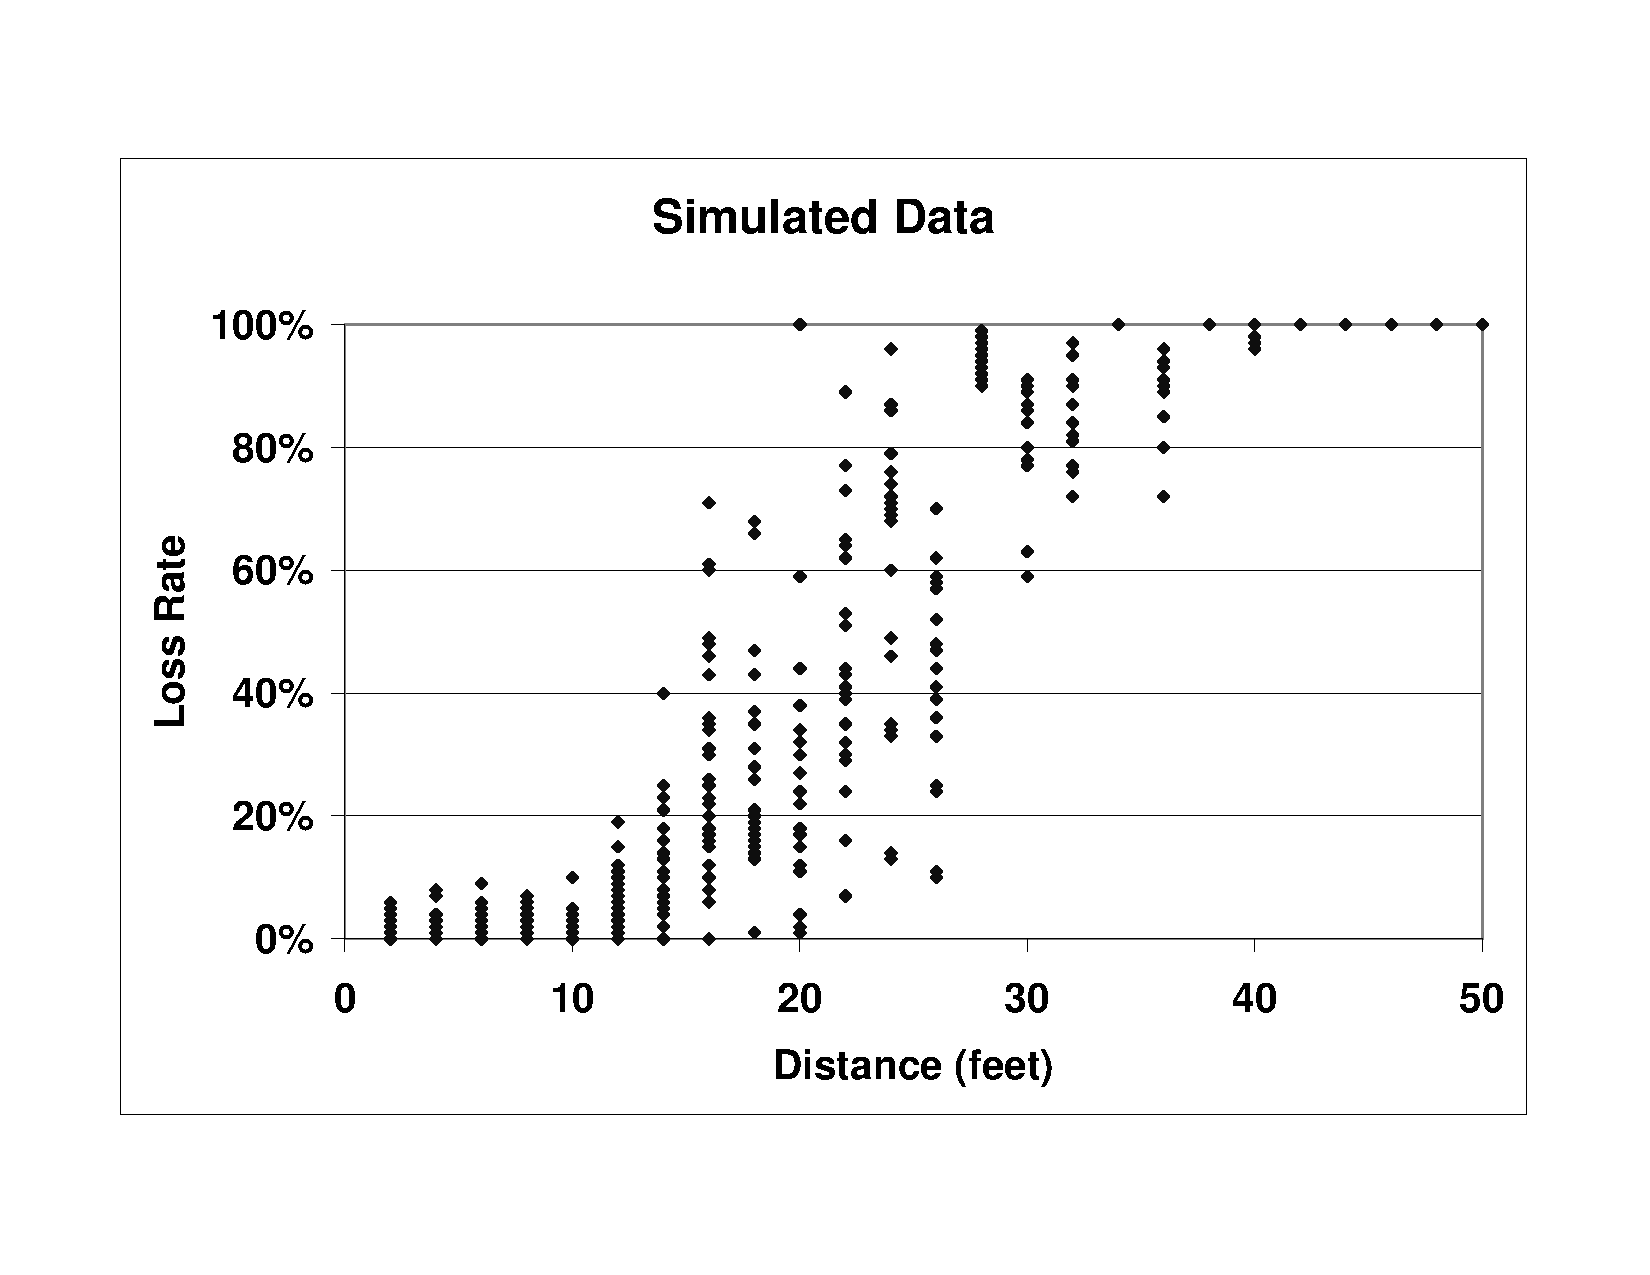
\includegraphics[clip,angle=-90,width=2in]{fig/simulated.pdf}}

\caption{Empirical and Corresponding Simulated Packet Loss Data}
\label{fig:loss_fig}
\end{figure}


The ``lossy'' radio model places the nodes in a directed graph. Each
edge $(a,b)$ in the graph means $a$'s signal can be heard by
$b$. Every edge has a value in the range $(0,1)$, representing the
probability a bit sent by $a$ will be corrupted (flipped) when $b$
hears it. For example, a value of 0.01 means each bit transmitted has
a 1\% chance of being flipped, while 1.0 means every bit will be
flipped, and 0.0 means bits will be transmitted without error. Each
bit is considered independently.

The graph of the lossy model can be specified at \sim boot with a
file. \sim looks for the file ``lossy.nss'' by default, but an
alternate file can be specified with the {\tt -rf} flag. The file has
the following format:

\begin{verbatim}
<mote ID>:<mote ID>:bit error rate
<mote ID>:<mote ID>:bit error rate
<mote ID>:<mote ID>:bit error rate ...
\end{verbatim}

For example,

\begin{verbatim}
0:1:0.012333
1:0:0.009112
1:2:0.013196
\end{verbatim}

\noindent specifies that mote 1 hears mote 0 with a bit error rate of 1.2\%,
mote 0 hears mote 1 with a bit error rate of 0.9\%, and mote 2 hears
mote 1 with a bit error rate of 1.3\%. By making the graph directed,
\sim can model asymmetric links, which initial empirical studies have
suggest are a common occurance in TinyOS RFM-stack networks.

By specifying error at the bit level, \sim can capture many causes of
packet loss and noise in a TinyOS network, including missed start
symbols, data corruption, and acknowledgement errors.

\sim includes a Java tool, {\tt net.tinyos.sim.LossyBuilder} for generating
loss rates from physical topologies.  The tool models loss rates
observed empirically in an experiment performed by Woo et al. on a
TinyOS network~\cite{empirical}.  The empirical data is from a network
of twenty-six \motes, placed in a line, spaced at regular two foot
intervals, with the TinyOS radio set at a medium power setting (50 out
of 100). Each \mote transmitted two hundred packets, with each other
\mote keeping track of the number of packets
heard. Figure~\ref{fig:loss_empirical} shows a plot of this empirical
data.

To generate lossy models, the tool has Gaussian packet loss
probability distributions for each distance, fit to match the
empirical data. Given a physical \mote topology, the tool generates
packet loss rates for each \mote pair by sampling these
distributions. The tool translates packet error rates into independent
bit error rates.  Figure~\ref{fig:loss_sim} shows the results of the
experiment used to gather loss data when run in \sim.

The lossy model models interference and corruption, but it does not
model noise; if no mote transmits, every mote will hear a perfectly
clear channel.

\subsection{Using LossyBuilder}

LossyBuilder assumes each mote has a transmission radius of 50
feet. Combined with the bit error rate, this means each mote transmits
its signal in a disc of radius 50 feet, with the bit error rate
increasing with distance from the center.

LossyBuilder can read in or generate physical topologies ((x,y)
coordinates), and generate loss topologies from physical topologies by
sampling from the model of the empirical distribution in
Figure~\ref{fig:loss_empirical}. Its usage is:

\begin{verbatim}
usage: java net.tinyos.sim.LossyBuilder [options]
options:
  -t grid:       Topology (grid only and default)
  -d <m> <n>:    Grid size (m by n) (default: 10 x 10)
  -s <scale>:    Spacing factor (default: 5.0)
  -o <file>:     Output file
  -i <file>:     Input file of positions
  -p:            Generate positions, not error rates
\end{verbatim}

Running LossyBuilder will, by default, generate a loss topology for a
10 by 10 grid with a grid spacing of five feet (45' by 45'), and print
it to standard out. It prints the loss topology in the form that \sim
expects. The {\tt -i} option allows you to specify an input file of
(x,y) positions, which has the format

\begin{verbatim}
x y
x y
x y ...
\end{verbatim}

\noindent where the coordinate system is in feet. The first (x,y) pair
is the position of mote 0, the second is the position of mote 1,
etc.

For example,

\begin{verbatim}
java net.tinyos.sim.LossyBuilder -d 20 20 -s 10 -o 20x20-10.nss
\end{verbatim}

\noindent will output a loss topology of a 20 by 20 grid, with
ten foot spacing, and write it to the file ``20x20-10.nss''.

\subsection{Bit Errors and Packet Errors}

The forumula for calculating packet error rates ($E_{p}$) from bit
error rates ($E_{b}$) for the mica RFM 40Kb stack with SecDed encoding
is:

\begin{eqnarray*}
&&E_{p} = 1 - (S_{s} \cdot (S_{e})^{d})\\
&&S_{s} = (1 - E_{b})^{9}\\
&&S_{e} = (1 - E_{b})^{8} + (8 \cdot E_{b} \cdot (1 - E_{b})^{12})\\
&&E_{p} = 1 - ((1 - E_{b})^{9} \cdot ((1 - E_{b})^{8} + (8 \cdot E_{b} \cdot (1 - E_{b})^{12}))^{d})
\end{eqnarray*}

where $S_{s}$ is the start symbol success probability, $S_{e}$ the
probability a packet byte is uncorrupted (zero or one bit errors), and
$d$ is the number of bytes in the packet.

The simple model can be represented in the lossy model: it is a fully
connected graph, in which every edge has a loss probability of
zero. However, doing so requires specifying the entire graph to \sim;
the simple model is an easy shortcut (and has an internal
representation that's more efficient).

\subsection{Lossy Model Actuation}

Specifying a loss topology with a file defines a static topology over
an entire simulation. There are simulation situations, however, in
which changing topologies are needed. \sim therefore allows users to
modify the loss topology at run-time. Applications can connect to \sim
over a TCP socket and send control messages to add, delete, or modify
network links. Currently, the only application that does so is
TinyViz, discussed in Section~\ref{sec:tinyviz}. The TinyViz network
plugins use the same empirical model of LossyBuilder to generate link
loss rates; moving motes causes TinyViz to send the appropriate
commands to \sim.

\section{ADC Models}
\label{sec:adc}

\begin{figure}
\centering
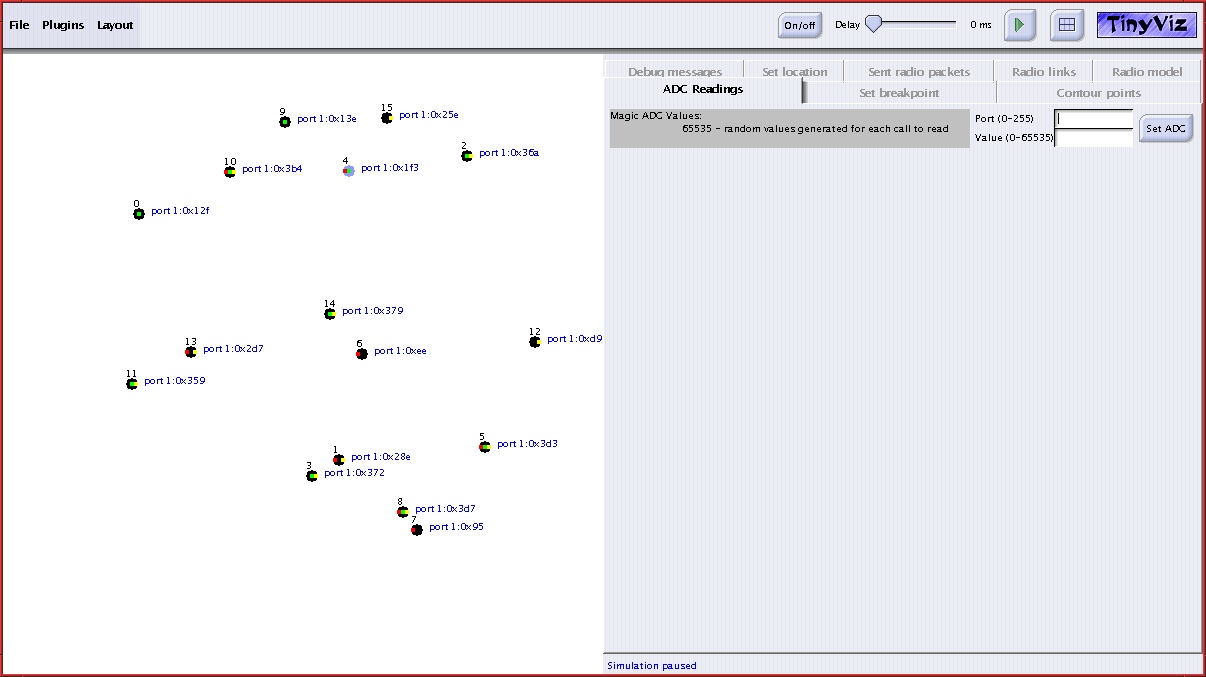
\includegraphics[width=6.5in]{fig/adc-viz.png}
\caption{Setting ADC values in \tinyviz}
\label{fig:adc-viz}
\end{figure}


\sim provides two ADC models: random and generic. The model chosen specifies
how readings taken from the ADC are generated. Whenever any channel in
the ADC is sampled in the random model, it returns a 10-bit random
value (the rene and mica ADCs are 10 bits).

The general model also provides random values by default, but has
added functionality. Just as external applications can actuate the
lossy network model, they can also actuate the generic ADC model using
the \sim control channel, setting the value for any ADC port on any
mote. Currently, only \tinyviz, (discussed in
Section~\ref{sec:tinyviz}) supports this, through the ADC
plugin. Left-clicking on a mote selects it; using the ADC panel, you
can set the 10-bit value read from any of the mote's ADC
ports. Figure~\ref{fig:adc-viz} shows a screenshot of this \tinyviz
functionality.

\section{EEPROM}
\label{sec:eeprom}

\sim models the EEPROM at the line (16-byte block) level. \sim models it
with a large, memory-mapped file. By default, this file is anonymous,
and disappears when a simulation ends. However, with the {\tt -ef}
option, a user can specify a named file to use; this allows the EEPROM
data to persist across multiple simulation invocations.


\section{\tinyviz}
\label{sec:tinyviz}

\tinyviz is a Java visualization and actuation environment for
\sim. The main \tinyviz class is a jar file,
{\tt tools/java/net/tinyos/sim/tinyviz.jar}. \tinyviz can be attached
to a running simulation. Also, \sim can be made to wait for \tinyviz
to connect before it starts up, with the {\tt -gui} flag. This allows
users to be sure that \tinyviz captures all of the events in a given
simulation.

\tinyviz is not actually a visualizer; instead, it is a framework in
which plugins can provide desired functionality. By itself, \tinyviz
does little besides draw motes and their LEDs. However, it comes with
a few example plugins, such as one that visualizes network traffic.

\begin{figure}
\centering
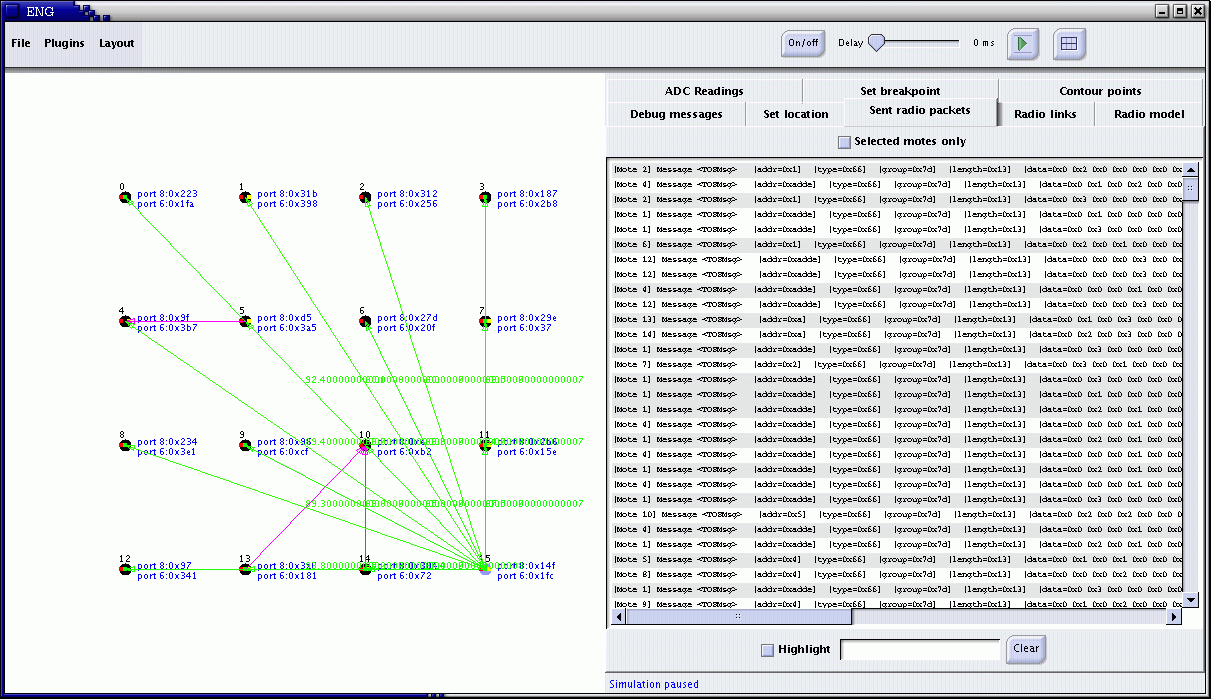
\includegraphics[width=6.5in]{fig/tinyviz.png}
\caption{\tinyviz connected to \sim running an object tracking
application. The right panel shows sent radio packets, the left panel
exhibits radio connectivity for \mote 15 and network traffic. The
green arrows and corresponding labels represent link probabilities for
\mote 15, and the magenta arrows indicate packet transmission.}
\label{fig:tinyviz}
\end{figure}

Figure~\ref{fig:tinyviz} shows a screenshot of the \tinyviz tool. The
left window contains the simulation visualization, showing 16 \motes
communicating in an ad-hoc network. The right window is the plugin
window; each plugin is a tab pane, with configuration controls and
data.

The second element on the top bar is the {\bf Plugin} menu, for
activating or de-activating individual plugins. Inactive plugins have
their tab panes greyed out.

The third element is the layout menu, which allows you to arrange
motes in specific topologies, as well as save or restore
topologies. \tinyviz can use physical topologies to generate network
topologies by sending messages to \sim that configure network
connectivity and the loss rate of individual links.

The right side of the top bar has three buttons and a slider. \tinyviz
can slow a simulation by introducing delays when it handles events
from \sim. The slider configures how long delays are. The On/Off
button turns selected motes on and off; this can be used to reboot a
network, or dynamically change its members. The button to the right of
the slider starts and stops a simulation; unlike the delays, which are
for short, fixed periods, this button can be used to pause a
simulation for arbitrary periods. The final button, on the far right,
enables and disables a grid in the visualization area. The small text
bar on the bottom of the right panel displays whether the simulation
is running or paused.

The \tinyviz engine uses an event-driven model, which allows easy
mapping between TinyOS' event-based execution and event-driven
GUIs. By itself, the application does very little; drop-in plugins
provide user functionality. \tinyviz has an event bus, which reads
events from a simulation and publishes them to all active plugins.

\subsection{\tinyviz Plugins}
\label{sec:plugins}

Users can write new plugins, which \tinyviz can dynamically load.  A
simple event bus sits in the center of \tinyviz; simulator messages
sent to \tinyviz appear as events, which any plugin can respond
to. For example, when a mote transmits a packet in \sim, the simulator
sends a packet send message to \tinyviz, which generates a packet send
event and broadcasts it on the event bus. A networking plugin can
listen for packet send events and update \tinyviz node state and draw
an animation of the communication.

Plugins can be dynamically registered and deregistered, which
correspondingly connect and disconnect the plugin from the event
bus. A plugin hears all events sent to the event bus, but individually
decides whether to do anything in response to a specific event; this
keeps the event bus simple, instead of having a content-specific
subscription mechanism.

A plugin must be a subclass of {\tt net.tinyos.sim.Plugin}. {\tt
Plugin} has the following signature:

\begin{verbatim}
public abstract class Plugin {

  public Plugin() {}

  public void initialize(TinyViz viz, JPanel pluginPanel) {...}
  public void register() {...}
  public void reset() { /* do nothing */}

  public abstract void deregister();
  public abstract void draw(Graphics graphics);
  public abstract void handleEvent(SimEvent event);
}
\end{verbatim}


Plugins register themselves with the \tinyviz event bus, which then
notifies them of all events coming in from TOSSIM; it is up to an
individual plugin whether to do something. The {\tt draw} method is
used to draw visualizations in the left pane of the TinyViz window.


\section{Using {\tt gdb}}

The binary executable produced by typing {\tt make pc} in any app
directory can be debugged using GDB. Developers of TinyOS code can
step through programs they have written, debugging deterministic,
logical aspects of their code before loading programs onto motes.

When accessing variables and functions in \sim under GDB, specific
prefixes precede them, to distinguish variables from different
components that have ths same name.  The nesC compiler takes each
component's fields and functions and renames them with unique
identifiers. This renaming for fields of a component is done by taking
the field name, and preceding it by the component name and a {\tt \$}
sign. Functions are renamed by taking the name of the function and
preceding it by the name of the component it is defined in, followed
by a {\tt \$} sign, followed by the interface name, followed by
another {\tt \$} sign.

The maximum number of nodes that can be simulated is determined at
compile time.  This value, as mentioned in section {\tt \sim
Architecture} specifies the size of the array for each component's
fields during code generation of the compilation process. When
compiling for the {\tt pc}, each declaration of a component field is
followed by {\tt [}, the value of {\tt tossim\_num\_nodes}, and {\tt
]}, where tossim\_num\_nodes is specified by the flag {\tt
-fnesc-tossim\_tosnodes=} in {\tt Makerules}, or by default, set to
1000.  This is the way \sim simulates multiple motes. \sim keeps an
array for each variable of state, and references each mote's
corresponding state when running code for that mote.

During code generation for the {\tt pc}, all references to component
fields are followed by {\tt [}, {\tt tos\_state.current\_node} and
{\tt ]}, where {\tt tos\_state.current\_node} refers to the moteID of
the mote \sim is currently executing code for.

For, for example, the {\tt Counter} component has a variable named
{\tt state} of type {\tt uint\_16t}. This translates to the C name
{\tt Counter\$state}. When compiled for \sim, it becomes {\tt
uint16\_t Counter\$state[MAX\_NODES]}. If a component has a variable
that's an array (e.g., {\tt uint8\_t buffer[8]}, it becomes an array of
arrays (e.g., {\tt uint8\_t buffer[8][MAX\_NODES]}). Laying out module
variables in this way means that overrun and underrun bugs will have
different effects on real motes and in TOSSIM. On a real mote, such a
bug will corrupt that mote's state; in TOSSIM, it will corrupt other
motes' state.

Using the application {\tt Blink} as an example, type {\tt make pc} in
the {\tt /apps/Blink/} directory to compile the application for
\sim. Run {\tt gdb} on the executable produced by typing {\tt gdb
build/pc/main.exe}. Examining {\tt BlinkM.td}, to break at the
function Clock.fire(), type {\tt break *BlinkM\$Clock\$fire}. {\tt
break} (or {\tt b}) specifies a breakpoint in GDB, and the {\tt *}
tells the GDB command line parser to examine the entire block of text
following it as a single expression. It is currently necessary to
specify the {\tt *} before the function name for GDB to parse it
properly. {\tt BlinkM} denotes the component the function is defined
in, and {\tt Clock} specifies the interface the function {\tt fire}
belongs to.

To run {\tt Blink} with one mote, type {\tt run 1} or {\tt r 1}.  {\tt
r} is the GDB command to run the current executable, and all values
after the {\tt r} are passed as arguments to the executable. Therefore
the {\tt 1} specifies the number of motes to simulate to \sim. MoteIDs
are assigned starting at 0.  In this current example the moteID of the
single mote being simulated is 0.

Upon hitting the breakpoint at {\tt fire}, to print the value of {\tt
BlinkM}'s {\tt state}, type \\{\tt print
BlinkM\$state[tos\_state.current\_node]} (or {\tt p} for {\tt
print}). {\tt p} is the print command in GDB. {\tt BlinkM} corresponds
to the component the field {\tt state} belongs to. Since the
application was compiled for the pc, it is necessary to specify which
mote's {\tt BlinkM\$state} to access, as {\tt
[tos\_state.current\_node]} following the field name does.

\section{Concurrency Model}

\sim captures the TinyOS event-driven concurrency model at interrupt and
task granularity. For a description of the TinyOS concurrency model,
refer to the TinyOS documentation. This document does not describe the
model, merely how \sim implements it.

\sim models each TinyOS interrupt as a simulation event. Each event is
associated with a specific mote. Simulator events run atomically with
respect to one another. Therefore, unlike on real hardware, interrupts
cannot pre-empt one another. After each simulator event executes, \sim
checks the task queue for any pending tasks, and executes all of them
in FIFO scheduling order. In \sim, interrrupts do not pre-empt tasks.
This method of task execution means that spinning tasks (e.g., tasks
that enqueue themselves in a spin-lock fashion) will cause \sim to
execute that task indefinitely. Using tasks in this way is contrary to
the event-driven TinyOS programming model.

Once a simulator event calls an interrupt handler, the handler
executes TinyOS code through commands and events.

\subsection{Sample Execution}

\begin{figure*}
\scriptsize
\centering
\begin{tabular}{ll}
Time (4MHz ticks) & Action \\ \hline
3987340 & Simulator event is dequeued and handled at time 3987340.\\
        & The clock interrupt handler is called, signaling the application Timer
 event.\\
        & \hspace{0.2in} {\it The application's Timer handler requests a reading
 from the ADC.}\\
        & The ADC component puts a simulator ADC event on the queue with timesta
mp 3987540.\\
        & The interrupt handler completes; the clock event re-enqueues itself fo
r the next tick.\\

3987540 & Simulator ADC event is dequeued and handled at time 3987540.\\
        & The ADC interrupt handler is called, signaling an ADC ready event with
 a sensor value.\\
        & \hspace{0.2in}{\it The application event handler takes the top three b
its and calls LEDs commands.}\\
        & The ADC interrupt handler completes.\\

7987340 & Simulator event is dequeued and handled at time 7987340.\\
        & The clock interrupt handler is called, signaling the application Timer
 event.\\
        & \ldots execution continues as above
\end{tabular}
\caption{Sample Execution}
\label{fig:exec}
\end{figure*}

Figure \ref{fig:exec} contains a sample execution that demonstrates
the workings of \sim. A simple program, {\tt SenseToLeds}, is running
on a single \mote. This program has a 1Hz timer that samples the light
sensor and displays the three high order bits of the reading on the
\mote LEDs. Since simulator time is kept in terms of a 4MHz clock, the
timer events are four million ticks apart, and the 50$\mu$s ADC
capture takes 200 ticks between request and interrupt. In Figure
\ref{fig:exec} \sim-specific
execution is shown in plain text, while unchanged TinyOS execution is
shown in italics. This sample execution shows how a small number of
\sim events results in the series of TinyOS events and commands
comprising an entire (albeit very simple) application.

\section{Internals}
\label{sec:internals}

Currently, \sim compiles by using alternative implementations of some
core system components (e.g. {\tt Main.nc}, {\tt HPLUART.nc}) and
incorporating a few extra files (e.g. {\tt event\_queue.c}).

The basic \sim structure definitions exist in {\tt
platform/pc/nido.h}. These include the global simulation state
(event queue, time, etc.) and individual node state. Hardware settings
that affect multiple components (such as the potentiometer setting)
currently must be modeled as global node state. {\tt nido.h} also
includes a few useful macros, such as {\tt NODE\_NUM} and {\tt
THIS\_NODE}; these should be used whenever possible, so minimal code
modifications will be necessary if the data representation
changes. 

{\tt Nido.nc} is where the \sim global state is defined. The {\tt
main()} function parses the command line options, initializes the
\sim global state, initializes the external communication
functionality (defined in {\tt external\_comm.c, PCRadio.h}), then
initializes the state of each of the simulated motes with {\tt call
StdControl.init()} and {\tt call StdControl.start()}. It then starts
executing a small loop that handles events and schedules tasks.

\subsection{\sim Architecture}

\sim replaces a small number of TinyOS components, the components
that handle interrupts and the {\tt Main} component. Interrupts are
modeled as simulatgor discrete events. Normally, the core TinyOS loop
that runs on motes is this:

\begin{verbatim}
while(1){
  TOSH_run_task();
}
\end{verbatim}

{\tt TOSH\_run\_task} runs tasks until the task queue is empty, at which
point it puts the CPU to sleep. An interrupt will wake the mote. If
the interrupt has caused a task to be scheduled, then that task will
be run. While that task is running, interrupts can be handled.

The core \sim loop is slightly different:

\begin{verbatim}
for (;;) {
  while(TOSH_run_next_task()) {}
  if (!queue_is_empty(&(tos_state.queue))) {	
    tos_state.tos_time =
       queue_peek_event_time(&(tos_state.queue));
    queue_handle_next_event(&(tos_state.queue));
}
\end{verbatim}


A notion of virtual time (stored as a 64-bit integer) is kept in the
simulator (stored in {\tt tos\_state.tos\_time}), and every event is
associated with a specific mote. Most events are emulations of
hardware interrupts. For example, when the clock in {\tt hpl.c} is
initialized to certain counter values, \sim's implementation
enqueues a clock interrupt event, whose handler calls the function
normally registered as the clock interrupt handler; from this point,
normal TinyOS code takes over (in terms of events being signaled,
etc.) In addition, the event enqueues another clock event for the
future, with its time (for the event queue) being the current time
plus the time between interrupts.

When compiling for \sim, the nesC compiler modifies code generation
for components such that fields declared in components result in
arrays of each field.  The maximum number of motes that can be
simulated at once is set at compile time by the size of this array;
the default value is 1000 and is specified in {\tt /apps/Makerules}
with the {\tt -fnesc-tossim-tosnodes=} flag. Since every event is
associated with a specific mote, the {\tt tos\_state.current\_node}
field is set just before the event handler function is called, so that
all modifications to component fields affect the correct mote's
state. Since all TinyOS tasks enqueued by an event are run to
completion before the next event is handled, tasks all execute with
the same node number and access the enqueuing mote's state.

\subsection{\sim Implementations}

To load a component, the nesC compiler uses a directory search
path. The default search path is:

\begin{itemize}
\item The application directory
\item {\tt tos/platform/xxx} (the selected platform)
\item {\tt tos/sensorboards/xxx} (the selected sensor board(s))
\item {\tt tos/system}
\item {\tt tos/lib}
\end{itemize}
Entries can be prepended to the search path with the {\tt -I} option
to the compiler. Using the {\tt -I} option therefore allows you to use
alternative implementations of components provided by TinyOS. For
example, one can write a \sim implementation of the microphone, and
put it in a separate directory, then include that directory with {\tt
-I}. This will cause the compiler to load the new \sim implementation
instead of the default one in the sensor board directory.

The component model of TinyOS means that \sim implementations are not
constrained to hardware abstractions. For example, \sim has an
implementation of the {\tt EEPROM} component, instead of the
lower-level hardware interface. Similarly, instead of using a
bit-level simulation, one can write a \sim implementation of {\tt
AMStandard}, for a packet-level simulation.

\subsection{RFM}

A \sim network model has the following structure:

\begin{verbatim}
typedef struct {
  void(*init)();
  void(*transmit)(int, char);   // int moteID, char bit
  void(*stop_transmit)(int);    // int moteID
  char(*hears)(int);            // char bit,   int moteID
  bool(*connected)(int,int);    // int moteID1, int moteID2
  link_t*(*neighbors)(int);      // int moteID
} rfm_model;
\end{verbatim}

{\tt init}, {\tt transmit}, {\tt stop\_transmit} and {\tt hears} are
straightforward; they're used to transmit and receive bits. The {\tt
connected} and {\tt neighbors} functions are used for some specific
low-level emulations of the radio channel during bit synchronization.

To give a feel for how the \sim RFM model works, we'll step through
the lossy model. The variable names have been changed to make it a bit
easier to explain.

In the lossy model, each mote has four variables: the value it
currently {\tt hears}, whether it is transmitting or not, and a
structure defining its network links. Each network link has a bit
error probability and stores the value currently being transmitted
along that link (after error).

Every time a mote {\tt transmit()}s (after error) a 1 to another mote,
that mote's {\tt hears} variable is incremented. When the transmitting
mote calls {\tt stop\_transmit()}, the variable is decremented. When
the receiver calls {\tt hears()}, it receives a 1 if the {\tt hears}
variable is non-zero. Signals are therefore modeled as a logical or.

When a mote transmits a zero or one with {\tt transmit()}, the
function scans through the list of network connections ({\tt
neighbors()}). For each link, it flips the bit with the probability
specified by that link, and stores the bit that's actually transmitted
(this is needed for when {\tt stop\_transmit()} is called, so {\tt
hears} can be decremented properly).

\bibliographystyle{unsrt}
\small

\begin{thebibliography}{99}
\bibitem{empirical}
\newblock{D.~Ganesan, B.~Krishnamachari, A.~Woo, D.~Culler, D.~Estrin, and  S.~Wicker.}
\newblock {An empirical study of epidemic algorithms in large scale multihop  wireless networks.}
\newblock {\url{citeseer.nj.nec.com/ganesan02empirical.html}, 2002.}
\newblock {Submitted for publication, February 2002.}

\bibitem{tossim}
\newblock{P.~Levis, N.~Lee, M.~Welsh, and D.~Culler.}
\newblock{TOSSIM: Accurate and Scalable Simulation of Entire TinyOS Applications}
\newblock{To appear in {\it Proceedings of the First ACM Conference on Embedded Networked Sensor Systems (SenSys 2003)}.}

\end{thebibliography}

\end{document}





